% ============================================================
% Question Bank: ch02-02 Connecting Percents and Proportions
% Topic Title: Connecting Percents and Proportions
% CCSS: 7.RP.A.3
% Questions: 30 (18 MC + 7 SA + 5 Graphical)
% ============================================================

% --- Multiple Choice Questions (18) ---

\begin{practiceQuestion}{2-2-q01}{mc}
\begin{questionText}
Which proportion can be used to find what percent $18$ is of $60$?
\end{questionText}
\choiceA{$\dfrac{18}{60} = \dfrac{p}{100}$}
\choiceB{$\dfrac{60}{18} = \dfrac{p}{100}$}
\choiceC{$\dfrac{p}{18} = \dfrac{60}{100}$}
\choiceD{$\dfrac{18}{100} = \dfrac{p}{60}$}
\correctAnswer{A}
\explanation{Part over whole equals percent over $100$: $\frac{18}{60} = \frac{p}{100}$.}
\end{practiceQuestion}

\begin{practiceQuestion}{2-2-q02}{mc}
\begin{questionText}
Use a proportion to find $35\%$ of $120$.
\end{questionText}
\choiceA{$35$}
\choiceB{$38$}
\choiceC{$42$}
\choiceD{$48$}
\correctAnswer{C}
\explanation{Set up $\frac{n}{120} = \frac{35}{100}$. Cross-multiply: $100n = 4200$. Divide: $n = 42$.}
\end{practiceQuestion}

\begin{practiceQuestion}{2-2-q03}{mc}
\begin{questionText}
$24$ out of $80$ students chose pizza for lunch. What percent is that?
\end{questionText}
\choiceA{$24\%$}
\choiceB{$28\%$}
\choiceC{$30\%$}
\choiceD{$32\%$}
\correctAnswer{C}
\explanation{$\frac{24}{80} = \frac{p}{100}$. Cross-multiply: $80p = 2400$. Divide: $p = 30\%$.}
\end{practiceQuestion}

\begin{practiceQuestion}{2-2-q04}{mc}
\begin{questionText}
Which proportion shows that $42$ is $60\%$ of some number $w$?
\end{questionText}
\choiceA{$\dfrac{42}{w} = \dfrac{60}{100}$}
\choiceB{$\dfrac{w}{42} = \dfrac{60}{100}$}
\choiceC{$\dfrac{60}{42} = \dfrac{w}{100}$}
\choiceD{$\dfrac{42}{60} = \dfrac{w}{100}$}
\correctAnswer{A}
\explanation{Part ($42$) over whole ($w$) equals percent ($60$) over $100$: $\frac{42}{w} = \frac{60}{100}$.}
\end{practiceQuestion}

\begin{practiceQuestion}{2-2-q05}{mc}
\begin{questionText}
Solve using a proportion: $72$ is $90\%$ of what number?
\end{questionText}
\choiceA{$64.8$}
\choiceB{$75$}
\choiceC{$78$}
\choiceD{$80$}
\correctAnswer{D}
\explanation{$\frac{72}{w} = \frac{90}{100}$. Cross-multiply: $90w = 7200$. Divide: $w = 80$.}
\end{practiceQuestion}

\begin{practiceQuestion}{2-2-q06}{mc}
\begin{questionText}
In a bag of $150$ marbles, $60$ are blue. What percent of the marbles are blue?
\end{questionText}
\choiceA{$25\%$}
\choiceB{$30\%$}
\choiceC{$35\%$}
\choiceD{$40\%$}
\correctAnswer{D}
\explanation{$\frac{60}{150} = \frac{p}{100}$. Cross-multiply: $150p = 6000$. Divide: $p = 40\%$.}
\end{practiceQuestion}

\begin{practiceQuestion}{2-2-q07}{mc}
\begin{questionText}
A school has $500$ students. If $68\%$ eat in the cafeteria, how many eat there? Use a proportion.
\end{questionText}
\choiceA{$320$}
\choiceB{$340$}
\choiceC{$350$}
\choiceD{$368$}
\correctAnswer{B}
\explanation{$\frac{n}{500} = \frac{68}{100}$. Cross-multiply: $100n = 34{,}000$. Divide: $n = 340$.}
\end{practiceQuestion}

\begin{practiceQuestion}{2-2-q08}{mc}
\begin{questionText}
$15$ is what percent of $125$?
\end{questionText}
\choiceA{$10\%$}
\choiceB{$12\%$}
\choiceC{$15\%$}
\choiceD{$18\%$}
\correctAnswer{B}
\explanation{$\frac{15}{125} = \frac{p}{100}$. Cross-multiply: $125p = 1500$. Divide: $p = 12\%$.}
\end{practiceQuestion}

\begin{practiceQuestion}{2-2-q09}{mc}
\begin{questionText}
Use the equation method to find $55\%$ of $180$.
\end{questionText}
\choiceA{$90$}
\choiceB{$95$}
\choiceC{$99$}
\choiceD{$108$}
\correctAnswer{C}
\explanation{$n = 0.55 \times 180 = 99$. The proportion method gives the same answer: $\frac{n}{180} = \frac{55}{100}$ → $n = 99$.}
\end{practiceQuestion}

\begin{practiceQuestion}{2-2-q10}{mc}
\begin{questionText}
$96$ is $80\%$ of what number?
\end{questionText}
\choiceA{$76.8$}
\choiceB{$100$}
\choiceC{$116$}
\choiceD{$120$}
\correctAnswer{D}
\explanation{$\frac{96}{w} = \frac{80}{100}$. Cross-multiply: $80w = 9600$. Divide: $w = 120$.}
\end{practiceQuestion}

\begin{practiceQuestion}{2-2-q11}{mc}
\begin{questionText}
A recipe uses $3$ cups of sugar out of $12$ cups of ingredients total. What percent is sugar?
\end{questionText}
\choiceA{$20\%$}
\choiceB{$25\%$}
\choiceC{$30\%$}
\choiceD{$36\%$}
\correctAnswer{B}
\explanation{$\frac{3}{12} = \frac{p}{100}$. Cross-multiply: $12p = 300$. Divide: $p = 25\%$.}
\end{practiceQuestion}

\begin{practiceQuestion}{2-2-q12}{mc}
\begin{questionText}
Sarah and Jake both solve ``What is $40\%$ of $75$?'' Sarah uses a proportion; Jake uses an equation. Which statement is true?
\end{questionText}
\choiceA{Only the proportion method works}
\choiceB{Only the equation method works}
\choiceC{Both methods give the same answer}
\choiceD{The methods give different answers}
\correctAnswer{C}
\explanation{Proportion: $\frac{n}{75} = \frac{40}{100}$ gives $n = 30$. Equation: $n = 0.40 \times 75 = 30$. Both give $30$.}
\end{practiceQuestion}

\begin{practiceQuestion}{2-2-q13}{mc}
\begin{questionText}
A town has $2{,}400$ households. A survey shows $78\%$ have internet access. How many households have internet?
\end{questionText}
\choiceA{$1{,}800$}
\choiceB{$1{,}848$}
\choiceC{$1{,}872$}
\choiceD{$1{,}920$}
\correctAnswer{C}
\explanation{$\frac{n}{2400} = \frac{78}{100}$. Cross-multiply: $100n = 187{,}200$. Divide: $n = 1{,}872$.}
\end{practiceQuestion}

\begin{practiceQuestion}{2-2-q14}{mc}
\begin{questionText}
$27$ out of $180$ students earned an A on the exam. What percent earned an A?
\end{questionText}
\choiceA{$12\%$}
\choiceB{$15\%$}
\choiceC{$18\%$}
\choiceD{$27\%$}
\correctAnswer{B}
\explanation{$\frac{27}{180} = \frac{p}{100}$. Cross-multiply: $180p = 2700$. Divide: $p = 15\%$.}
\end{practiceQuestion}

\begin{practiceQuestion}{2-2-q15}{mc}
\begin{questionText}
Which equation is equivalent to the proportion $\dfrac{n}{250} = \dfrac{16}{100}$?
\end{questionText}
\choiceA{$n = 250 \div 16$}
\choiceB{$n = 16 \times 250$}
\choiceC{$100n = 250 \times 16$}
\choiceD{$16n = 250 \times 100$}
\correctAnswer{C}
\explanation{Cross-multiply: $100 \times n = 250 \times 16$, which gives $100n = 4000$.}
\end{practiceQuestion}

\begin{practiceQuestion}{2-2-q16}{mc}
\begin{questionText}
$135$ is $54\%$ of what number?
\end{questionText}
\choiceA{$72.9$}
\choiceB{$200$}
\choiceC{$245$}
\choiceD{$250$}
\correctAnswer{D}
\explanation{$\frac{135}{w} = \frac{54}{100}$. Cross-multiply: $54w = 13{,}500$. Divide: $w = 250$.}
\end{practiceQuestion}

\begin{practiceQuestion}{2-2-q17}{mc}
\begin{questionText}
There are $360$ students in a school. $45\%$ are boys. How many girls are in the school?
\end{questionText}
\choiceA{$162$}
\choiceB{$180$}
\choiceC{$195$}
\choiceD{$198$}
\correctAnswer{D}
\explanation{Boys: $0.45 \times 360 = 162$. Girls: $360 - 162 = 198$. Alternatively, girls are $55\%$: $0.55 \times 360 = 198$.}
\end{practiceQuestion}

\begin{practiceQuestion}{2-2-q18}{mc}
\begin{questionText}
A classroom has $28$ students. $7$ of them wear glasses. What percent wear glasses?
\end{questionText}
\choiceA{$20\%$}
\choiceB{$25\%$}
\choiceC{$28\%$}
\choiceD{$35\%$}
\correctAnswer{B}
\explanation{$\frac{7}{28} = \frac{p}{100}$. Cross-multiply: $28p = 700$. Divide: $p = 25\%$.}
\end{practiceQuestion}

% --- Short Answer Questions (7) ---

\begin{practiceQuestion}{2-2-q19}{sa}
\begin{questionText}
Use a proportion to find $85\%$ of $260$.
\end{questionText}
\correctAnswer{$221$}
\explanation{$\frac{n}{260} = \frac{85}{100}$. Cross-multiply: $100n = 22{,}100$. Divide: $n = 221$.}
\end{practiceQuestion}

\begin{practiceQuestion}{2-2-q20}{sa}
\begin{questionText}
$48$ is what percent of $320$?
\end{questionText}
\correctAnswer{$15\%$}
\explanation{$\frac{48}{320} = \frac{p}{100}$. Cross-multiply: $320p = 4800$. Divide: $p = 15\%$.}
\end{practiceQuestion}

\begin{practiceQuestion}{2-2-q21}{sa}
\begin{questionText}
$91$ is $65\%$ of what number?
\end{questionText}
\correctAnswer{$140$}
\explanation{$\frac{91}{w} = \frac{65}{100}$. Cross-multiply: $65w = 9100$. Divide: $w = 140$.}
\end{practiceQuestion}

\begin{practiceQuestion}{2-2-q22}{sa}
\begin{questionText}
A school garden has $80$ plants. If $45\%$ are tomato plants, how many tomato plants are there?
\end{questionText}
\correctAnswer{$36$}
\explanation{$\frac{n}{80} = \frac{45}{100}$. Cross-multiply: $100n = 3600$. Divide: $n = 36$ tomato plants.}
\end{practiceQuestion}

\begin{practiceQuestion}{2-2-q23}{sa}
\begin{questionText}
In a survey, $51$ out of $300$ people chose vanilla ice cream. What percent chose vanilla?
\end{questionText}
\correctAnswer{$17\%$}
\explanation{$\frac{51}{300} = \frac{p}{100}$. Cross-multiply: $300p = 5100$. Divide: $p = 17\%$.}
\end{practiceQuestion}

\begin{practiceQuestion}{2-2-q24}{sa}
\begin{questionText}
$156$ is $120\%$ of what number?
\end{questionText}
\correctAnswer{$130$}
\explanation{$\frac{156}{w} = \frac{120}{100}$. Cross-multiply: $120w = 15{,}600$. Divide: $w = 130$.}
\end{practiceQuestion}

\begin{practiceQuestion}{2-2-q25}{sa}
\begin{questionText}
A farmer harvested $420$ apples. He sold $315$ of them. What percent did he sell?
\end{questionText}
\correctAnswer{$75\%$}
\explanation{$\frac{315}{420} = \frac{p}{100}$. Cross-multiply: $420p = 31{,}500$. Divide: $p = 75\%$.}
\end{practiceQuestion}

% --- Graphical Questions (3 GMC + 2 GSA) ---

\begin{practiceQuestion}{2-2-q26}{gmc}
\begin{questionText}
The table below shows the results of a class vote for a field trip. What percent of the class voted for the zoo?

\begin{center}
\begin{tabular}{|l|c|}
\hline
\textbf{Destination} & \textbf{Votes} \\
\hline
Zoo & $18$ \\
\hline
Museum & $12$ \\
\hline
Aquarium & $15$ \\
\hline
Park & $15$ \\
\hline
\end{tabular}
\end{center}
\end{questionText}
\choiceA{$18\%$}
\choiceB{$25\%$}
\choiceC{$30\%$}
\choiceD{$36\%$}
\correctAnswer{C}
\explanation{Total votes: $18 + 12 + 15 + 15 = 60$. Zoo: $\frac{18}{60} = \frac{p}{100}$ → $p = 30\%$.}
\end{practiceQuestion}

\begin{practiceQuestion}{2-2-q27}{gmc}
\begin{questionText}
The bar model below represents a whole amount. Use the model to find what percent the shaded part is of the whole.

\begin{center}
\begin{tikzpicture}[scale=0.65]
  % Whole bar divided into 8 equal parts, 3 shaded
  \foreach \i in {0,...,7} {
    \draw[thick] (\i*1,0) rectangle (\i*1+1,0.8);
  }
  \fill[funBlue!40] (0,0) rectangle (1,0.8);
  \fill[funBlue!40] (1,0) rectangle (2,0.8);
  \fill[funBlue!40] (2,0) rectangle (3,0.8);
  \foreach \i in {0,...,7} {
    \draw[thick] (\i*1,0) rectangle (\i*1+1,0.8);
  }
  \draw[thick,<->] (0,-0.4) -- (3,-0.4) node[midway,below,font=\small] {$45$};
  \draw[thick,<->] (0,-1.1) -- (8,-1.1) node[midway,below,font=\small] {Whole $= {?}$};
  \node[above,font=\small] at (1.5,0.8) {Shaded};
\end{tikzpicture}
\end{center}

If each section has the same value and there are $8$ equal sections total, what percent is shaded?
\end{questionText}
\choiceA{$25\%$}
\choiceB{$33\%$}
\choiceC{$37.5\%$}
\choiceD{$45\%$}
\correctAnswer{C}
\explanation{$3$ out of $8$ sections are shaded. $\frac{3}{8} = \frac{p}{100}$ → $p = 37.5\%$.}
\end{practiceQuestion}

\begin{practiceQuestion}{2-2-q28}{gmc}
\begin{questionText}
Look at the proportion model below. What value of $n$ makes the proportion true?

\begin{center}
\begin{tikzpicture}[scale=0.7]
  % Two bars representing the proportion
  % Top bar: n out of 80
  \draw[thick] (0,1.5) rectangle (8,2.3);
  \fill[funGreen!40] (0,1.5) rectangle (3,2.3);
  \draw[thick] (0,1.5) rectangle (8,2.3);
  \draw[thick] (3,1.5) -- (3,2.3);
  \node[above,font=\small] at (1.5,2.3) {$n$};
  \node[above,font=\small] at (5.5,2.3) {};
  \node[right,font=\small] at (8.2,1.9) {$80$};
  % Bottom bar: percent out of 100
  \draw[thick] (0,0) rectangle (10,0.8);
  \fill[funGreen!40] (0,0) rectangle (3.75,0.8);
  \draw[thick] (0,0) rectangle (10,0.8);
  \draw[thick] (3.75,0) -- (3.75,0.8);
  \node[below,font=\small] at (1.875,0) {$37.5$};
  \node[right,font=\small] at (10.2,0.4) {$100$};
  % Connection
  \node[font=\small] at (-0.5,1.15) {$=$};
\end{tikzpicture}
\end{center}
\end{questionText}
\choiceA{$28$}
\choiceB{$30$}
\choiceC{$32$}
\choiceD{$37.5$}
\correctAnswer{B}
\explanation{$\frac{n}{80} = \frac{37.5}{100}$. Cross-multiply: $100n = 3000$. Divide: $n = 30$.}
\end{practiceQuestion}

\begin{practiceQuestion}{2-2-q29}{gsa}
\begin{questionText}
The double number line below shows a percent relationship. What number goes at the question mark?

\begin{center}
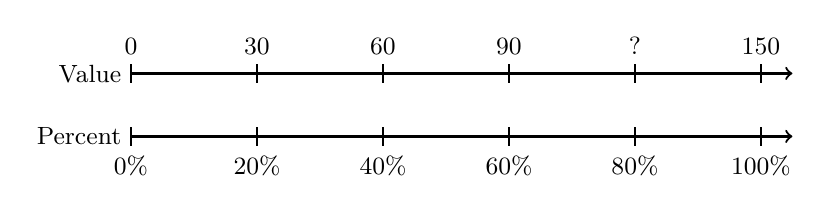
\begin{tikzpicture}[scale=0.8]
  % Top number line (values)
  \draw[thick,->] (0,1) -- (10.5,1);
  \node[left,font=\small] at (0,1) {Value};
  \foreach \x/\lab in {0/0, 2/30, 4/60, 6/90, 8/?, 10/150} {
    \draw[thick] (\x,0.85) -- (\x,1.15);
    \node[above,font=\small] at (\x,1.15) {\lab};
  }
  % Bottom number line (percent)
  \draw[thick,->] (0,0) -- (10.5,0);
  \node[left,font=\small] at (0,0) {Percent};
  \foreach \x/\lab in {0/0\%, 2/20\%, 4/40\%, 6/60\%, 8/80\%, 10/100\%} {
    \draw[thick] (\x,-0.15) -- (\x,0.15);
    \node[below,font=\small] at (\x,-0.15) {\lab};
  }
\end{tikzpicture}
\end{center}
\end{questionText}
\correctAnswer{$120$}
\explanation{The whole ($100\%$) corresponds to $150$. At $80\%$: $\frac{n}{150} = \frac{80}{100}$ → $n = 120$.}
\end{practiceQuestion}

\begin{practiceQuestion}{2-2-q30}{gsa}
\begin{questionText}
The model below shows that a number $w$ is split into a shaded part and an unshaded part. The shaded part is $84$ and represents $70\%$ of the whole. What is the whole number $w$?

\begin{center}
\begin{tikzpicture}[scale=0.6]
  % Bar model
  \fill[funBlue!40] (0,0) rectangle (7,1);
  \draw[thick] (0,0) rectangle (10,1);
  \draw[thick] (7,0) -- (7,1);
  \node[font=\small] at (3.5,0.5) {$84$};
  \node[font=\small] at (8.5,0.5) {?};
  \draw[thick,<->] (0,-0.5) -- (7,-0.5) node[midway,below,font=\small] {$70\%$};
  \draw[thick,<->] (0,-1.3) -- (10,-1.3) node[midway,below,font=\small] {$w = {?}$};
\end{tikzpicture}
\end{center}
\end{questionText}
\correctAnswer{$120$}
\explanation{$\frac{84}{w} = \frac{70}{100}$. Cross-multiply: $70w = 8400$. Divide: $w = 120$.}
\end{practiceQuestion}
